% ===============================================================
% Appendix: backup slides (dataset, metric formulas, parameters,
% detailed results, qualitative outputs).
% ===============================================================
\section*{Appendix}

% ----- Dataset and fine-tuning ---------------------------------
\begin{frame}{Appendix: Dataset and Fine-Tuning}
\begin{itemize}
  \item \textbf{Clip:} Sanbapolis basketball, three synchronised cameras (cam\_13, cam\_2, cam\_4).
  \item \textbf{Length:} 525 frames at 25\,fps ($\approx 21$\,s).
  \item \textbf{Ground truth:} 2D boxes annotated every fifth frame; intrinsics provided.
  \item \textbf{Detector training:} separate disjoint clip, from YOLO26m weights.
  \item \textbf{Schedule:} up to 300 epochs (patience 30), 1280\,px input, batch size 4.
\end{itemize}
\end{frame}

% ----- Metric formulas: detection and tracking -----------------
\begin{frame}{Appendix: Metric Formulas (Detection and Tracking)}
\textbf{Detection}
\[
\text{Prec} = \frac{TP}{TP+FP}, \quad
\text{Rec} = \frac{TP}{TP+FN}, \quad
F_1 = \frac{2\,\text{Prec}\cdot\text{Rec}}{\text{Prec}+\text{Rec}}, \quad
\text{IoU} = \frac{|A \cap B|}{|A \cup B|}
\]
\textbf{Tracking} \;{\footnotesize(TP, FP, FN from matching at localization threshold $\alpha$; HOTA integrates over $\alpha$)}
\[
\text{IDF1} = \frac{2\,IDTP}{2\,IDTP + IDFP + IDFN}, \qquad
\text{HOTA} = \int_0^1 \sqrt{\text{DetA}_\alpha\cdot\text{AssA}_\alpha}\;\,d\alpha
\]
\[
\text{DetA}_\alpha = \frac{|TP|}{|TP|+|FN|+|FP|}, \qquad
\text{AssA}_\alpha = \frac{1}{|TP|}\sum_{c\,\in\,TP} A(c)
\]
\[
A(c) = \frac{|TPA(c)|}{|TPA(c)|+|FNA(c)|+|FPA(c)|}, \qquad
\text{LocA} = \frac{1}{|TP|}\sum_{c\,\in\,TP}\text{IoU}(c)
\]
\end{frame}

% ----- Metric formulas: 3D and trajectory ----------------------
\begin{frame}{Appendix: Metric Formulas (3D and Trajectory)}
\textbf{Reprojection error} (3D point $X_i$ projected by camera $P$, observed at $x_i$)
\[
e_i = \lVert x_i - \pi(P, X_i)\rVert, \qquad
\text{RMSE} = \sqrt{\tfrac{1}{N}\textstyle\sum_i e_i^{2}}
\]
\textbf{Trajectory error} (prediction $p_t$, ground truth $g_t$, over $T$ frames)
\[
\text{ADE} = \frac{1}{T}\sum_{t=1}^{T}\lVert p_t - g_t\rVert, \quad
\text{FDE} = \lVert p_T - g_T\rVert, \quad
\text{MTE} = \operatorname{median}_t \lVert p_t - g_t\rVert
\]
\end{frame}

% ----- Parameters: MOG2 and YOLO -------------------------------
\begin{frame}{Appendix: Pipeline Parameters (Detection)}
\scriptsize
\begin{columns}[T]
  \begin{column}{0.48\textwidth}
    \centering MOG2 and preprocessing\\[2pt]
    \begin{tabular}{lr}
      \toprule
      Parameter & Value \\
      \midrule
      Learning rate            & $-1$ (adaptive) \\
      Detect shadows           & off \\
      CLAHE clip limit         & 6.0 \\
      CLAHE tile grid          & $8\times8$ \\
      Min.\ blob area (px$^2$) & 500 \\
      Max.\ blob area (px$^2$) & 10000 \\
      \bottomrule
    \end{tabular}
  \end{column}
  \begin{column}{0.48\textwidth}
    \centering YOLO detection and NMS\\[2pt]
    \begin{tabular}{lr}
      \toprule
      Parameter & Value \\
      \midrule
      \multicolumn{2}{l}{\textit{Single-pass}} \\
      \quad Confidence       & 0.3 \\
      \quad Inference size   & 640 \\
      \quad Built-in NMS IoU & 0.45 \\
      \multicolumn{2}{l}{\textit{Two-pass fine-tuned}} \\
      \quad Player size (px) & 1280 \\
      \quad Ball size (px)   & 1600 \\
      \quad Ball confidence  & 0.2 \\
      \quad Merge NMS IoU    & 0.75 \\
      \bottomrule
    \end{tabular}
  \end{column}
\end{columns}
\end{frame}

% ----- Parameters: tracking and geometry -----------------------
\begin{frame}{Appendix: Pipeline Parameters (Tracking and Geometry)}
\scriptsize
\begin{columns}[T]
  \begin{column}{0.48\textwidth}
    \centering Tracking (DeepSORT)\\[2pt]
    \begin{tabular}{lr}
      \toprule
      Parameter & Value \\
      \midrule
      Max.\ IoU distance        & 0.7 \\
      Max.\ appearance distance & 0.2 \\
      Max.\ age (frames)        & 60 \\
      Confirmation hits         & 2 \\
      Feature budget            & 100 \\
      Coast age (frames)        & 5 \\
      Resurrection window       & 150 \\
      OSNet embedding dim       & 512 \\
      \bottomrule
    \end{tabular}
  \end{column}
  \begin{column}{0.48\textwidth}
    \centering Geometry\\[2pt]
    \begin{tabular}{lr}
      \toprule
      Parameter & Value \\
      \midrule
      Max.\ interpolated gap     & 5 \\
      EMA weight $\alpha$        & 0.5 \\
      Ground inlier gate (mm)    & 600 \\
      Ball reproj.\ gate (px)    & 30 \\
      Minimum views              & 2 \\
      Mahalanobis gate ($\chi^2$) & 11.345 \\
      Position noise (mm)        & 30 \\
      Measurement noise (mm)     & 80 \\
      \bottomrule
    \end{tabular}
  \end{column}
\end{columns}
\end{frame}

% ----- Detailed results: detection -----------------------------
\begin{frame}{Appendix: Detection Results}
\footnotesize
\centering
\begin{tabular}{llrrrr}
\toprule
Method & Camera & Precision & Recall & $F_1$ & Mean IoU \\
\midrule
\multirow{3}{*}{MOG2}
  & cam\_13 & 0.471 & 0.262 & 0.337 & 0.651 \\
  & cam\_2  & 0.345 & 0.408 & 0.374 & 0.663 \\
  & cam\_4  & 0.328 & 0.293 & 0.309 & 0.700 \\
\midrule
\multirow{3}{*}{YOLO pre-trained}
  & cam\_13 & 0.851 & 0.617 & 0.716 & 0.754 \\
  & cam\_2  & 0.858 & 0.778 & 0.816 & 0.782 \\
  & cam\_4  & 0.922 & 0.801 & 0.857 & 0.808 \\
\midrule
\multirow{3}{*}{YOLO fine-tuned}
  & cam\_13 & 0.872 & 0.732 & 0.796 & 0.758 \\
  & cam\_2  & 0.835 & 0.761 & 0.796 & 0.757 \\
  & cam\_4  & 0.923 & 0.822 & 0.870 & 0.796 \\
\bottomrule
\end{tabular}
\end{frame}

% ----- Detailed results: tracking ------------------------------
\begin{frame}{Appendix: Tracking Results}
\footnotesize
\centering
\setlength{\tabcolsep}{4.5pt}
\begin{tabular}{llrrrrrrr}
\toprule
Tracker & Camera & IDP & IDR & IDF1 & HOTA & DetA & AssA & LocA \\
\midrule
\multirow{3}{*}{SORT}
  & cam\_13 & 0.660 & 0.514 & 0.590 & 0.438 & 0.484 & 0.398 & 0.797 \\
  & cam\_2  & 0.743 & 0.607 & 0.668 & 0.517 & 0.515 & 0.522 & 0.794 \\
  & cam\_4  & 0.768 & 0.605 & 0.679 & 0.542 & 0.575 & 0.514 & 0.829 \\
\midrule
\multirow{3}{*}{DeepSORT}
  & cam\_13 & 0.588 & 0.533 & 0.569 & 0.434 & 0.469 & 0.405 & 0.769 \\
  & cam\_2  & 0.617 & 0.603 & 0.610 & 0.480 & 0.453 & 0.511 & 0.761 \\
  & cam\_4  & 0.670 & 0.605 & 0.638 & 0.521 & 0.553 & 0.495 & 0.798 \\
\bottomrule
\end{tabular}
\end{frame}

% ----- Detailed results: 3D geometry ---------------------------
\begin{frame}{Appendix: 3D Geometry Errors}
\footnotesize
\centering
\setlength{\tabcolsep}{3pt}
\begin{tabular}{lrrrrrrrrr}
\toprule
& \multicolumn{6}{c}{Reprojection error} & \multicolumn{3}{c}{Trajectory error} \\
\cmidrule(lr){2-7}\cmidrule(lr){8-10}
Camera & Mean & Median & RMSE & Acc@25 & Acc@50 & Acc@100 & ADE & FDE & MTE \\
\midrule
cam\_13 & 499.6 & 300.5 &  844.9 & 0.087 & 0.134 & 0.219 &  9976.1 &  8503.9 & 10662.2 \\
cam\_2  & 772.5 & 459.6 & 1378.8 & 0.023 & 0.038 & 0.076 &  3984.4 &  5098.8 &  4373.3 \\
cam\_4  & 395.3 & 176.0 &  905.4 & 0.188 & 0.247 & 0.359 &  8636.7 &  7238.4 &  8739.9 \\
\bottomrule
\end{tabular}
\vspace{0.5em}
\par\footnotesize Errors in mm; Acc columns are fractions at 25, 50, 100\,mm. Fragment counts: 2, 5, 5.
\end{frame}

% ----- Qualitative outputs (stacked vertically) ----------------
\begin{frame}{Appendix: Qualitative Outputs, Detection (1/2)}
\centering
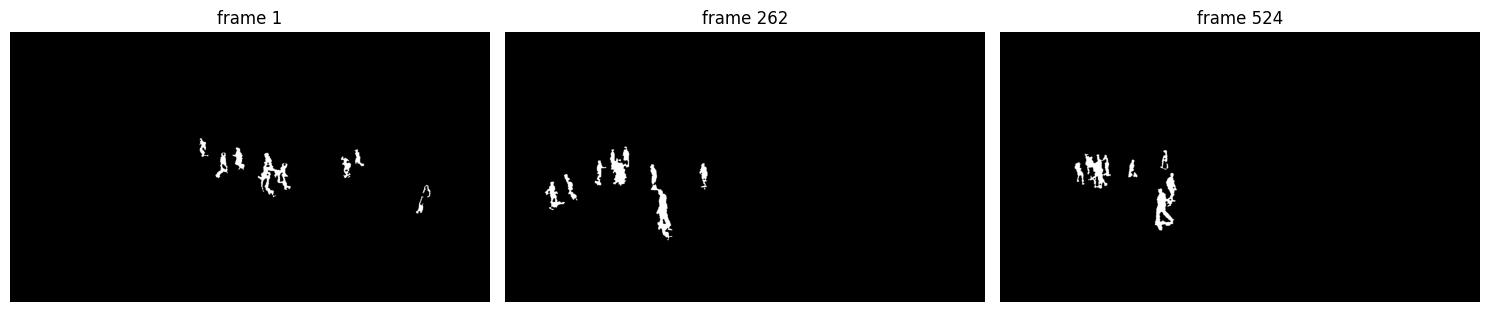
\includegraphics[width=0.92\textwidth]{../assets/media/appendix/02_inspect_mog2_detections.png}\\
{\scriptsize MOG2 foreground mask}\\[1.2em]
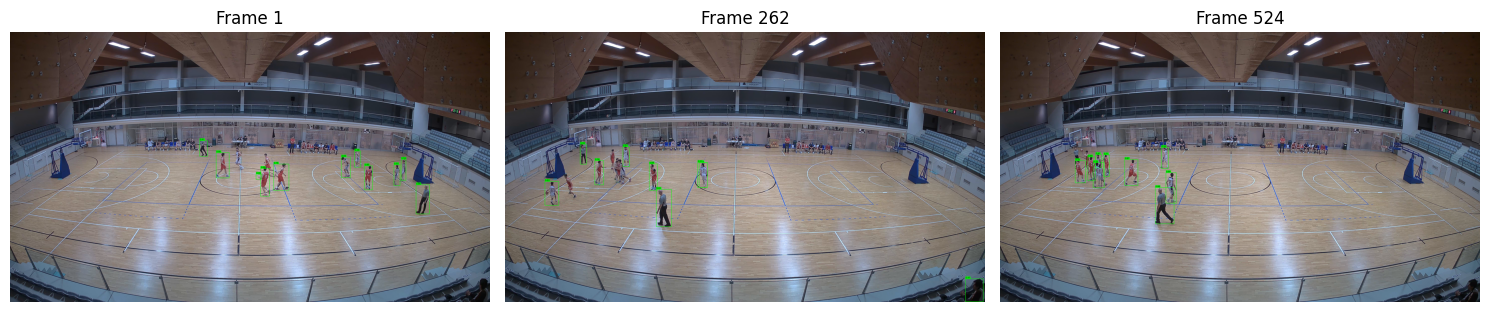
\includegraphics[width=0.92\textwidth]{../assets/media/appendix/04_inspect_yolo_detections.png}\\
{\scriptsize Pre-trained YOLO26 detections}
\end{frame}

\begin{frame}{Appendix: Qualitative Outputs, Detection (2/2)}
\centering
\vfill
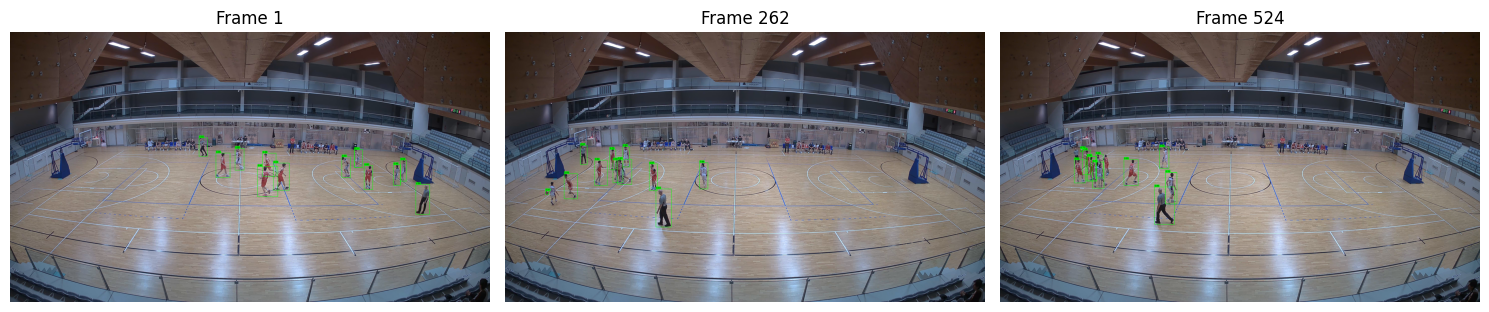
\includegraphics[width=0.92\textwidth]{../assets/media/appendix/05_inspect_merged_detections.png}\\
{\scriptsize Fine-tuned YOLO26, merged dual-pass detections}
\vfill
\end{frame}

\begin{frame}{Appendix: Qualitative Outputs, Tracking}
\centering
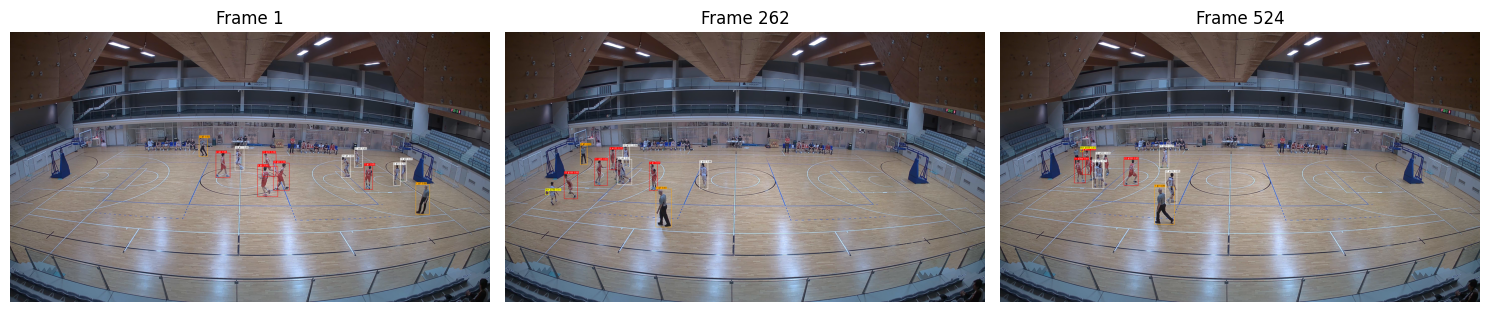
\includegraphics[width=0.92\textwidth]{../assets/media/appendix/07_inspect_sort_tracks.png}\\
{\scriptsize SORT tracks}\\[1.2em]
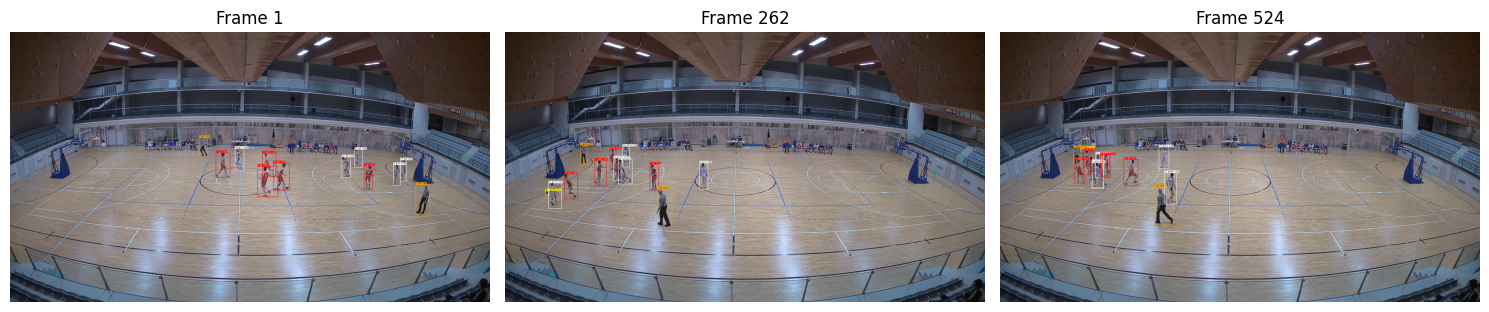
\includegraphics[width=0.92\textwidth]{../assets/media/appendix/10_inspect_resolved_labels.png}\\
{\scriptsize DeepSORT tracks after label resolution}
\end{frame}

\begin{frame}{Appendix: Qualitative Outputs, 3D Reconstruction}
\centering
\vfill
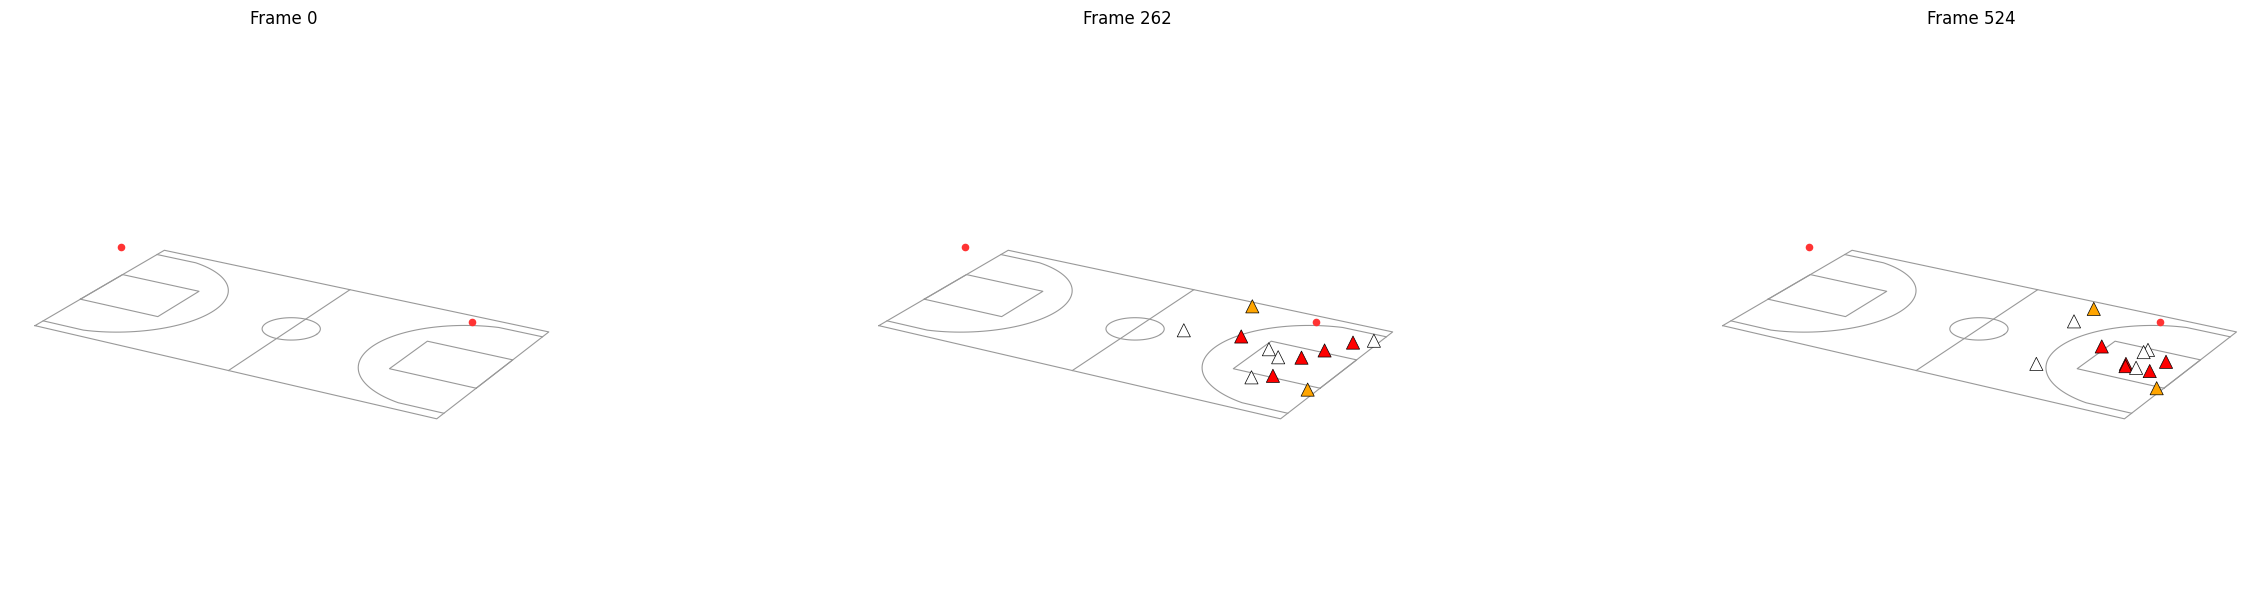
\includegraphics[width=0.92\textwidth]{../assets/media/appendix/12_inspect_smoothed_3d_reconstructions.png}\\
{\scriptsize Smoothed 3D reconstruction}
\vfill
\end{frame}
